\section{Dealing with variation}
\label{imaging:variation}


Experimental error is always present in our
measurements. Additionally, any given feature
may show extensive biological variability even within
apparently homogeneous populations. The biological
variation can be informative, as it gives us
insight into the limits to accuracy of cellular
processing and can reveal phenotypically distinct
subpopulations (see \ar{insulation:introduction}).
However, if experimental error is mis-interpreted
as biological variability, we lose statistical resolution
or may assign unwarranted meaning to non-biological
variation. It is then important to be able to separate
experimental from biological variation.


Experimental variation in fluorescence imaging
comes from many sources.
The imaging plane itself may cause
variation by intersecting cells at different
relative heights. This focal plane effect
can cause cell-to-cell differences in the
degree of focus and in how much off-plane
fluorescence is captured. As discussed
in \ar{imaging:distortion}, image shading and
background can also contribute to artificial variation
due to microscopy.


Aside from microscopy artifacts, the process
of preparing cells for imaging may also
generate distortions of true biological variability.
For example, variation in cellular surface
area or volume may lead to differences
in how well an antibody or non-permeable dye
can access an intracellular target.
Such differences in cell morphology may be
enhanced or dampened by fixatives, which can cause cells to shrink
in the $z$-axis \cite{Pawly2006}.


  \begin{figure}[!bt]
  \centering
  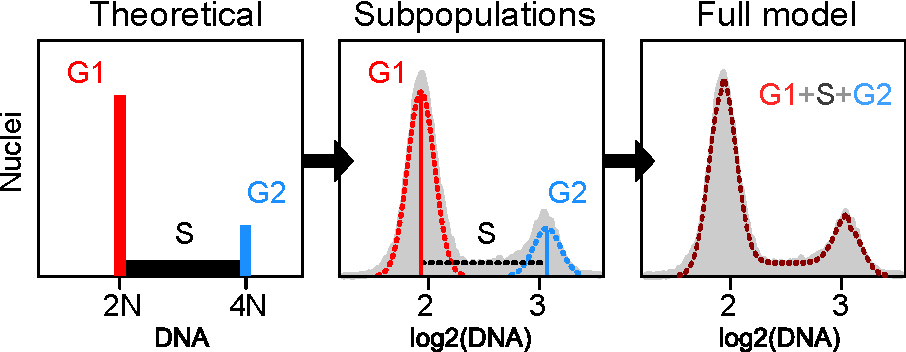
\includegraphics[width=4in]{FIGS/imaging/cycleFit.pdf}
  {\singlespacing 
  \caption[ Fitting total DNA to a simple cell cycle model.]
            {An asynchronous cell population can be
            fit to a simple model of the cell cycle
            with reasonable accuracy. Left,
            the theoretical
            asynchronous cell-cycle distribution consists
            of delta functions for G1 and G2 cells (i.e.
            all cells in these populations have identical
            DNA content) and a uniform distribution for
            S-phase cells that are moving from the G1 to G2
            states at a constant rate. Middle, the
            total DNA feature of G1 and G2 nuclei shows log-normal variation
            that can thus be fit to normal distributions after log-transformation.
            Right, the cell subpopulation models 
            add up to a reasonably accurate estimate
            of the cell cycle distribution. Gray, filled
            histograms are of $\log_2$(total DNA), with 
            DNA in arbitrary units, of $\sim2\times10^4$ Hoechst-stained
            human colonic epithelial cells. Dashed lines are
            the actual fits to this data using the method described
            in the text.}
  \label{fig:imaging:cycleFit}}
  \end{figure}


Finally, non-biological variation can be introduced
during segmentation. This can be due to outright errors
(e.g. a cell being split into two objects) or to
the more subtle fact that the accuracy of a set of
segmentation parameters will vary from cell to cell.
For example, a chosen threshold that perfectly separates
background from foreground for one cell may end up
discarding the outer edges of a dimmer cell.


\subsection{Using DNA features for quality control}
\label{imaging:variation:dnaQC}

Due to the error sources discussed above (among others)
there may be many outlier cells to discard. Manual or pseudo-manual
approaches are often used for this task. 
Visual inspection of a random
subset of segmented cells is a common approach,
though automated solutions are needed for large datasets.
An example is the identification of out-of-focus images using
image-level features from tools like PhenoRipper
\cite{Rajaram2012}.
I use an automated statistical approach that takes
advantage of ``ground truth'' aspects of total DNA
content in cells. 
This approach uses population-level statistics
of DNA features to determine which cells
are likely to be properly
segmented and in focus. In effect, I make the assumption that
cells with biologically-unlikely DNA feature values will have
non-biological values in other features as well.




  \begin{figure}[!bt]
  \centering
  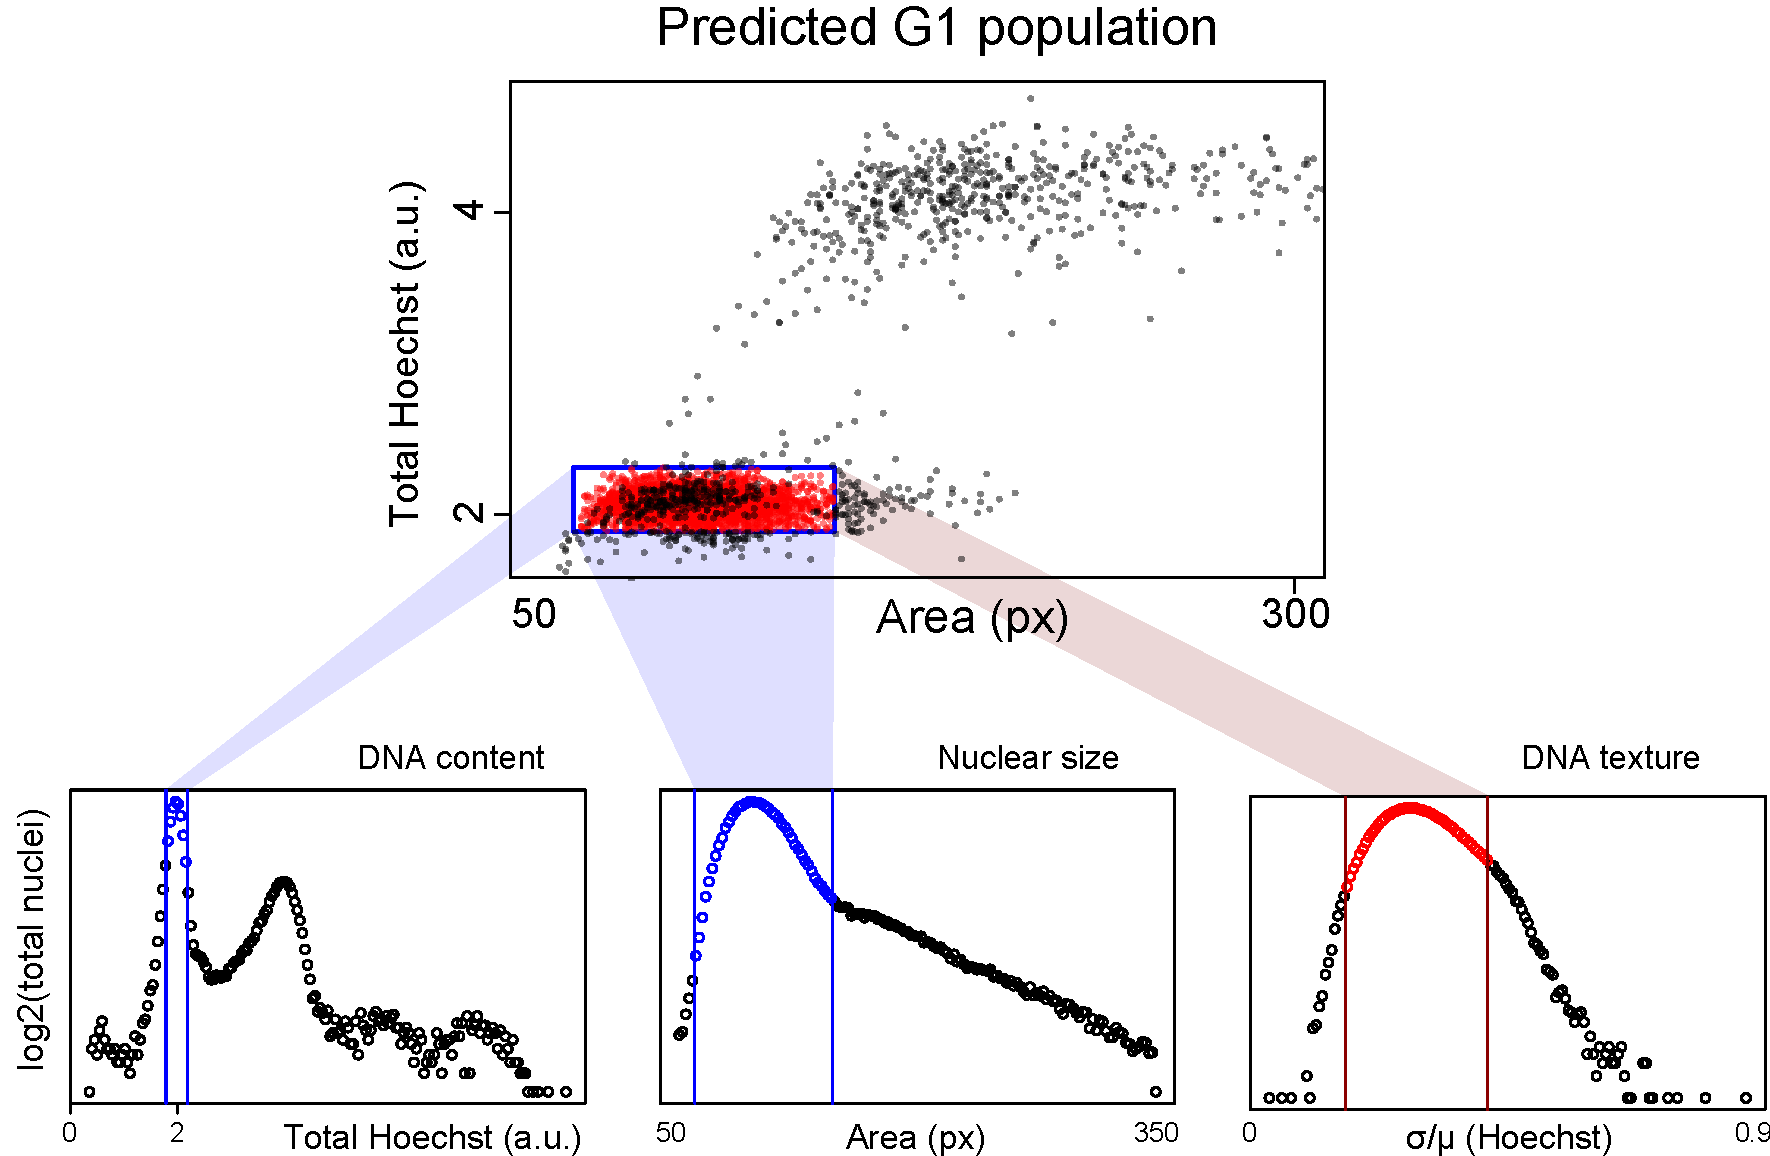
\includegraphics[width=6in]{FIGS/imaging/qualityControl.pdf}
  {\singlespacing 
  \caption[ Using DNA features for quality control.]
            {DNA features can be used for single-cell quality
            control. Bottom left, the Total DNA feature
            is fit to a cell cycle plot (fit not shown)
            and the G1 population is gated as all cells
            within $\mu_{G1}\pm2\sigma_{G1}$ (blue). The population is
            also statistically gated using the nuclear area (bottom,
            middle) and the intra-nuclear intensity $cv$ (bottom, right).
            The gating is $\pm3\times\text{MAD}$ from the median of each
            feature, where $\text{MAD}$ is the median absolute deviation
            ($\text{median}(|X-\text{median}(X)|)$. 
            ($3\times\text{MAD}\approx2\sigma$ for normal distributions.)
            The gated points are considered to be in-focus G1 cells
            that are likely segmented properly. In the top plot,
            these quality-controlled
            cells are found as red points within the blue box. Data from
            >4000 Hoechst-stained human colonic epithelial cells.}
  \label{fig:imaging:qualityControl}}
  \end{figure}



The first step in my quality control pipeline is to identify cell cycle
subpopulations by fitting a cell cycle model
to the total DNA histograms. This allows for later isolation
of these subpopulations and removal of outliers. Note that
in tissue culture microscopy
mitotic (M-phase) cells are often lost during sample washes
and so are already excluded from analysis.


An asynchronous cell population can be accurately
fit to a simple model of the cell cycle. The
theoretical, variation-free model of this cell cycle
consists of of delta functions for the G1 and G2 peaks
with a uniform S-phase distribution in between
(\ar{fig:imaging:cycleFit}, left). In other words, all
cells within G1 or G2 have the exact same DNA content,
and cells moving through S-phase increase their DNA content
at a constant rate. In reality,
the cell cycle distribution arising from measured
total DNA consists of $\log$-normally distributed G1
and G2 peaks, with a variable-shaped S-phase distribution
in between. I note that, on a $\log$-scale, the G1 and
G2 distributions have near-identical standard deviations
($\sigma_{G1}\approx\sigma_{G2}$).



I implemented a simple variant of the
Dean-Jett-Fox cell cycle model \cite{Dean1974,Fox1980}
that is sufficient to accurately identify G1 and G2 cells
from microscopy data.
The formulae that comprise this model are in
Equations~\ref{eq:imaging:g1}\nobreakdash-\ref{eq:imaging:g2},
where: $T_c$ is the $\log_2$-transformed
total DNA of a single cell; $\mu_{G1}$ is the average of this
value across all G1-phase cells; $\sigma$ is the standard
deviation of the G1 and G2 distributions; $v$ is the height of the S-phase
uniform distribution, $f(T_c)$ is the fraction of
cells with the same $T_c$ DNA content (in practice, it is the fraction of cells
falling into the same histogram bin), and $w$ values are weights. \ar{fig:imaging:cycleFit} shows
this model graphically, fit to experimental data.
    %
    \begin{align}
    f_{G1}(T_c) &= \frac{w_1}{\sigma \sqrt{2\pi}}
    e^{-\frac{(T_c-\mu_{G1})^2}{2\sigma^2}} \label{eq:imaging:g1}\\
    f_{S} (T_c) &= \left\{
        \begin{array}{lr}
        0 & : T_c \notin [ \mu_{G1}, \mu_{G2} ] \\
        v & : T_c \in    [ \mu_{G1}, \mu_{G2} ]
        \end{array}
        \right.
    \label{eq:imaging:s}\\
    f_{G2}(T_c) &= \frac{w_2}{\sigma \sqrt{2\pi}}
    e^{-\frac{(T_c-\mu_{G2})^2}{2\sigma^2}} \label{eq:imaging:g2}
    \end{align}


While fitting to a cell cycle distribution model may
be sufficient to identify biological outlier cells, I use two
additional DNA features to further exclude low-quality
images of nuclei. These features
are the nuclear area and the coefficient of variation ($cv$)
of intra-nuclear DNA intensity.
The $cv$ is a rough proxy for the DNA texture,
and so can be used to identify out-of-focus cells
(lower $cv$) or those with chromatin condensation or
punctate artifacts (higher $cv$). I therefore statistically
gate the population by rejecting those cells that are too
far from the median of either of these features
(see \ar{fig:imaging:qualityControl}).


Finally, I restrict my analyses to cells in the G1 phase
\arp{fig:imaging:qualityControl}.
The rationale for this is that I do not expect G1
and G2 cells to have different qualitative behaviors
for the signaling pathways that I study in \ar{insulation:introduction},
though I do expect them to have somewhat different quantitative
behaviors. The effect of combining these subpopulations
would then be a meaningless increase in apparent signaling variability.
I therefore chose the G1 population as it is
typically more populated and is less prone to
double-segmentation errors.


\subsection{Using DNA features to correct measurement error}


By using DNA features for quality control, we can thus collect
all cells within the G1 and/or G2 populations that are high-quality
(from an imaging standpoint) and accurately segmented.
The quality control described above may be a sufficient level of
data clean-up for some experimental goals, but
it does not deal with the problem
identified at the top of this section: 
that is, the separation of true biological variation from
measurement error. In other words, quality control only discards
cells that are too far from the ``typical'' cell, it does nothing
to determine or correct the measurement error in those cells that are kept.


To identify biological variability, then,
I again take advantage of the cell cycle ``ground truth.''
As shown in \ar{fig:imaging:cycleFit}, the theoretical
cell cycle distribution has no variation in the G1 or G2
populations, as all cells have exactly the same diploid
or tetraploid DNA content. The observed variation
around the theoretical values then do not carry any biological
meaning. (Note that this approximation becomes less accurate
with chromosomally-unstable cell populations.)


\subsubsection{Single-cell measurement error correction}
\label{imaging:singleCellCorrection}

If the variation in total DNA carries no biological
information, then it should not be predictive of
of other feature values: any feature dependence on
the DNA content must then be due to a global source
of error. In principle, then, we can then reduce this error by 
removing the meaningless correlations of other features to total DNA content. 


  \begin{figure}[!bt]
  \centering
  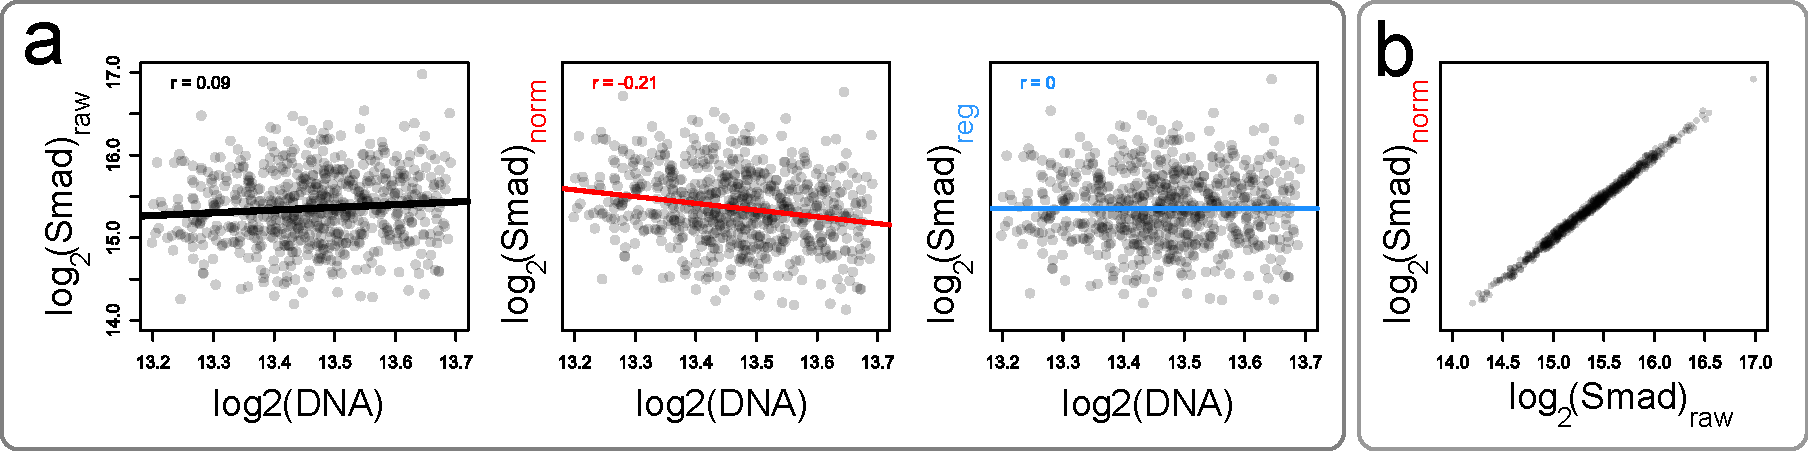
\includegraphics[width=6in]{FIGS/imaging/singleCellNorm.pdf}
  {\singlespacing 
  \caption[ Single-cell correction using DNA features.]
            {The variation in total DNA content (within a single cell cycle peak)
            is non-biological and therefore should not be predictive of
            intensity values for other probes.
            \b{a}, Total Smad as a function of
            total DNA. The raw data show a low
            Pearson correlation coefficient (inset $r$ value)
            and linear regression slope (black line),
            which is over-corrected by
            multiplicative normalization (middle) and
            corrected by regression-based normalization
            (right). \b{b}, Comparison of single-cell values
            before (x-axis) and after (y-axis) regresson-based
            correction. This dataset has low correlation to
            total DNA, and so the change is small. 
            $n=689$ human colonic epithelial cells (G1 only,
            quality-controlled) immunostained
            with anti-Smad2/3 (Smad) and Hoechst (DNA).
            All $y$-axes on the same scale.}
  \label{fig:imaging:singleCellNorm}}
  \end{figure}

I take two single-cell level approaches to correcting
total intensity feature errors
\arp{fig:imaging:singleCellNorm}. The intuitive method
is to estimate a normalization factor for e.g. all G1 cells
using total DNA ($T_{\text{DNA},c}$), and then use this
factor to normalize the total intensity of other
fluorescent probes ($T_{\text{probe},c}$)
in those same cells (\ar{eq:imaging:dnaNorm}). Indeed,
I have seen this approach used in the literature even
without first restricting analysis to one cell cycle
subpopulation. This
method assumes a simple multiplicative relationship
between the DNA and other channels such that, for example, a 10\%
increase in total DNA content would predict a 10\%
increase in different total probe intensity. Note
that this assumption may not hold true, such that this
method can cause over- or under-correction (as in
\ref{fig:imaging:singleCellNorm}a, middle).
    %
    \begin{equation} \label{eq:imaging:dnaNorm}
    f_{\text{norm}}(T_{\text{probe},c})=
    \frac{\text{median}_c(T_{\text{DNA},c})}{T_{\text{DNA},c}}T_{\text{probe},c}
    \end{equation}

    
My preferred method is regression-based, as it
guarantees removal of
correlation between total Hoechst and the total intensity of
another probe (\ar{fig:imaging:singleCellNorm}a, right).
For this method, linear regression is performed to get the
function in \ar{eq:imaging:reg} with slope $m$ and intercept $b$.
This results in a residual value ($\text{r}_{\text{probe},c}$)
for every cell.
The value of each $T_{\text{probe},c}$ can then be corrected
by setting it equal to the median across all values plus the residual
value for the same cell (\ar{eq:imaging:regNorm}).
    %
    \begin{gather}
    T_{\text{probe},c}=f_\text{regression}(T_{\text{DNA},c})=mT_{\text{DNA},c}+\text{r}_{\text{probe},c}+b
        \label{eq:imaging:reg}\\
    f_\text{norm}(T_{\text{probe},c}) =
        \text{median}_c(T_{\text{probe},c})+\text{r}_{\text{probe},c}
        \label{eq:imaging:regNorm}
    \end{gather}

    
For the sample data in \ar{fig:imaging:singleCellNorm} it is
clear that there is low basal correlation between total DNA
and total Smad, though I have observed much
higher correlations in some datasets. I further note that this same rationale
could be extended to non-DNA references and other features
for cases in which cross-probe
correlations are expected to be meaningless.
For all datasets in this dissertation I
apply the total DNA regression-based correction when accurate
single-cell values are needed (such as for the calculation of mutual
information between single-cell distributions).


\subsubsection{Population-level error correction}


While the single-cell correction above can be used to remove
those measurement errors that are directly shared by each probe,
it is reasonable to expect that much
of measurement error is more random and so affects probes independently. Though it is
not possible to correct single-cell values for such
unpredictable error, we can apply correction at the
population level.


  \begin{figure}[!bt]
  \centering
  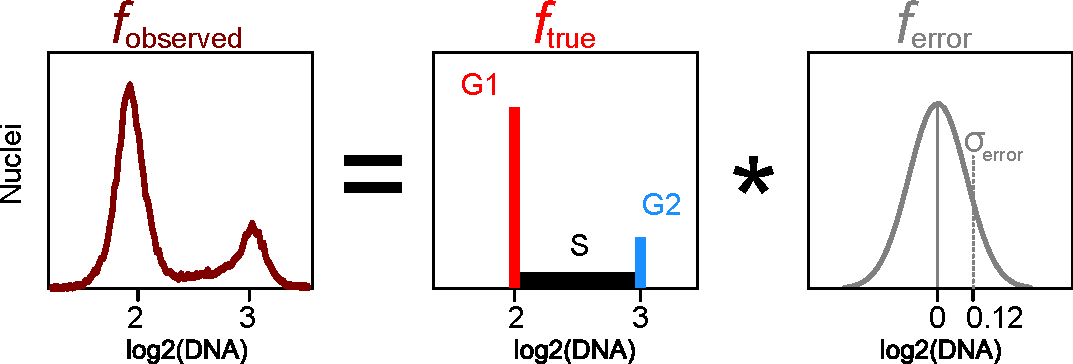
\includegraphics[width=4in]{FIGS/imaging/convolution.pdf}
  {\singlespacing 
  \caption[ Estimating measurement error of the total intensity feature.]
            {An observed total intensity distribution $f_\text{observed}$
            is the result of convolution of the true distribution
            $f_\text{true}$ and the measurement error $f_\text{error}$.
            The error function for total nuclear intensity features
            can be estimated as having $\sigma_\text{error}\approx
            \sigma_\text{DNA}$.
            Cartoon, using distributions from \ar{fig:imaging:cycleFit}.}
  \label{fig:imaging:convolution}}
  \end{figure}


An observed feature distribution can be modeled as the convolution
of a true biological distribution with a measurement error
distribution centered on zero, $f_{true}*f_{error}$. In the case of $\log$-total DNA
in G1 cells, $f_{true}$
is a delta distribution, $\delta_{true}$, positioned at $\mu_{G1}$.
I can then take advantage of
the property that $\delta_{true}*f_{error}=f_{error}+\mu_{G1}$.
In other words, the G1 and G2 distributions are themselves
estimates of the measurement error distribution, if their
means are set to 0
\arp{fig:imaging:convolution}.


For distributions that are log-normal, as are the total
intensity features for all probes used in this dissertation,
I can also use the property that two convolved normal distributions
yield a third normal distribution with mean
$\mu_3=\mu_1+\mu_2$ and variance
$\sigma_3^2=\sigma_1^2+\sigma_2^2$.
Thus, I can estimate the ``true'' cell-to-cell
total nuclear intensity variation
for any probe by \ar{eq:imaging:decon}. There of course may
be other sources of error not compensated for in this way, and
such an approach is only defensible for the total intensity feature.
    %
    \begin{equation} \label{eq:imaging:decon}
    \sigma_\text{probe,true} = \sqrt{ \sigma_\text{probe,observed}^2-\sigma_\text{DNA,error}^2 }
    \end{equation}

    
What utility does this deconvolution have? Published
measurements of cell-to-cell
variability range from 15-30\% \cite{Sigal2006a},
and my own raw data show values within
this same range. However, these values include measurement error
that is not being compensated for. Thus,
cell-to-cell variability, as measured by microscopy, is
necessarily overestimated. The above reasoning shows that
this overestimation is simple to measure, as all that is
needed are the log-scale standard deviations of the G1/2
total DNA distributions and the standard deviations of
the total-probe values in question.


I have not performed a comprehensive
study of the size of this effect, though I have measured it
in several independent datasets for various markers. I find
that deconvolved total intensity distributions yield
$\sim10\%$ lower standard deviations and $\sim10\%$ higher
information content (measured by mutual information \cite{Cheong2011}).
These inaccuracies are small enough that I feel comfortable
stating that measurement errors in high-quality microscopy datasets
are much smaller
than true biological variation.


It is important to note
that this DNA-based deconvolution makes the assumption
that the sources of error are the same between Hoechst and other probes. It is
possible that nuclear antibody-based stains have a partially non-overlapping
set of error sources with small molecules like Hoechst.
One possibility to address this, then, would be to use a
non-specific secondary antibody in a free channel.
That non-specific antibody should
not be correlated with the specific antibody staining in other
channels, and so any measured correlations could be removed using the
same rationale as for DNA content-based correction. Unfortunately,
I have had limited success with this
approach, though non-specific secondary antibodies
do indeed show high single-cell correlation. The problem has been that they also
show unexpected properties, like differences in intracellular
localization, for which adequate controls are not clear.

